\let\negmedspace\undefined
\let\negthickspace\undefined
\documentclass[a4,12pt,twocolumn]{IEEEtran}
%\documentclass[conference]{IEEEtran}
%\IEEEoverridecommandlockouts
% The preceding line is only needed to identify funding in the first footnote. If that is unneeded, please comment it out.
\usepackage{cite}
\usepackage{amsmath,amssymb,amsfonts,amsthm}
\usepackage{algorithmic}
\usepackage{graphicx}
\usepackage{textcomp}
\usepackage{xcolor}
\usepackage{txfonts}
\usepackage{listings}
\usepackage{enumitem}
\usepackage{mathtools}
\usepackage{gensymb}
\usepackage[breaklinks=true]{hyperref}
\usepackage{tkz-euclide} % loads  TikZ and tkz-base
\usepackage{listings}
\usepackage{empheq}
%
%\usepackage{setspace}
%\usepackage{gensymb}
%\doublespacing
%\singlespacing

%\usepackage{graphicx}
%\usepackage{amssymb}
%\usepackage{relsize}
%\usepackage[cmex10]{amsmath}
%\usepackage{amsthm}
%\interdisplaylinepenalty=2500
%\savesymbol{iint}
%\usepackage{txfonts}
%\restoresymbol{TXF}{iint}
%\usepackage{wasysym}
%\usepackage{amsthm}
%\usepackage{iithtlc}
%\usepackage{mathrsfs}
%\usepackage{txfonts}
%\usepackage{stfloats}
%\usepackage{bm}
%\usepackage{cite}
%\usepackage{cases}
%\usepackage{subfig}
%\usepackage{xtab}
%\usepackage{longtable}
%\usepackage{multirow}
%\usepackage{algorithm}
%\usepackage{algpseudocode}
%\usepackage{enumitem}
%\usepackage{mathtools}
%\usepackage{tikz}
%\usepackage{circuitikz}
%\usepackage{verbatim}
%\usepackage{tfrupee}
%\usepackage{stmaryrd}
%\usetkzobj{all}
%    \usepackage{color}                                            %%
\usepackage{array}                                            %%
%    \usepackage{longtable}                                        %%
%    \usepackage{calc}                                             %%
%    \usepackage{multirow}                                         %%
%    \usepackage{hhline}                                           %%
%    \usepackage{ifthen}                                           %%
  %optionally (for landscape tables embedded in another document): %%
%    \usepackage{lscape}     
%\usepackage{multicol}
%\usepackage{chngcntr}
%\usepackage{enumerate}

%\usepackage{wasysym}
%\newcounter{MYtempeqncnt}
\DeclareMathOperator*{\Res}{Res}
%\renewcommand{\baselinestretch}{2}
\renewcommand\thesection{\arabic{section}}
\renewcommand\thesubsection{\thesection.\arabic{subsection}}
\renewcommand\thesubsubsection{\thesubsection.\arabic{subsubsection}}

\renewcommand\thesectiondis{\arabic{section}}
\renewcommand\thesubsectiondis{\thesectiondis.\arabic{subsection}}
\renewcommand\thesubsubsectiondis{\thesubsectiondis.\arabic{subsubsection}}

% correct bad hyphenation here
\hyphenation{op-tical net-works semi-conduc-tor}
\def\inputGnumericTable{}                                 %%

\lstset{
%language=C,
frame=single, 
breaklines=true,
columns=fullflexible
}
%\lstset{
%language=tex,
%frame=single, 
%breaklines=true
%}

\begin{document}
%


\newtheorem{theorem}{Theorem}[section]
\newtheorem{problem}{Problem}
\newtheorem{proposition}{Proposition}[section]
\newtheorem{lemma}{Lemma}[section]
\newtheorem{corollary}[theorem]{Corollary}
\newtheorem{example}{Example}[section]
\newtheorem{definition}[problem]{Definition}
%\newtheorem{thm}{Theorem}[section] 
%\newtheorem{defn}[thm]{Definition}
%\newtheorem{algorithm}{Algorithm}[section]
%\newtheorem{cor}{Corollary}
\newcommand{\BEQA}{\begin{eqnarray}}
\newcommand{\EEQA}{\end{eqnarray}}
\newcommand{\define}{\stackrel{\triangle}{=}}

\bibliographystyle{IEEEtran}
%\bibliographystyle{ieeetr}


\providecommand{\mbf}{\mathbf}
\providecommand{\pr}[1]{\ensuremath{\Pr\left(#1\right)}}
\providecommand{\qfunc}[1]{\ensuremath{Q\left(#1\right)}}
\providecommand{\sbrak}[1]{\ensuremath{{}\left[#1\right]}}
\providecommand{\lsbrak}[1]{\ensuremath{{}\left[#1\right.}}
\providecommand{\rsbrak}[1]{\ensuremath{{}\left.#1\right]}}
\providecommand{\brak}[1]{\ensuremath{\left(#1\right)}}
\providecommand{\lbrak}[1]{\ensuremath{\left(#1\right.}}
\providecommand{\rbrak}[1]{\ensuremath{\left.#1\right)}}
\providecommand{\cbrak}[1]{\ensuremath{\left\{#1\right\}}}
\providecommand{\lcbrak}[1]{\ensuremath{\left\{#1\right.}}
\providecommand{\rcbrak}[1]{\ensuremath{\left.#1\right\}}}
\theoremstyle{remark}
\newtheorem{rem}{Remark}
\newcommand{\sgn}{\mathop{\mathrm{sgn}}}
%\providecommand{\abs}[1]{\left\vert#1\right\vert}
\providecommand{\res}[1]{\Res\displaylimits_{#1}} 
%\providecommand{\norm}[1]{\left\lVert#1\right\rVert}
%\providecommand{\norm}[1]{\lVert#1\rVert}
\providecommand{\mtx}[1]{\mathbf{#1}}
%\providecommand{\mean}[1]{E\left[ #1 \right]}
\providecommand{\fourier}{\overset{\mathcal{F}}{ \rightleftharpoons}}
%\providecommand{\hilbert}{\overset{\mathcal{H}}{ \rightleftharpoons}}
\providecommand{\system}{\overset{\mathcal{H}}{ \longleftrightarrow}}
	%\newcommand{\solution}[2]{\textbf{Solution:}{#1}}
\newcommand{\solution}{\noindent \textbf{Solution: }}
\newcommand{\cosec}{\,\text{cosec}\,}
\providecommand{\dec}[2]{\ensuremath{\overset{#1}{\underset{#2}{\gtrless}}}}
\newcommand{\myvec}[1]{\ensuremath{\begin{pmatrix}#1\end{pmatrix}}}
\newcommand{\mydet}[1]{\ensuremath{\begin{vmatrix}#1\end{vmatrix}}}
%\numberwithin{equation}{section}
%\numberwithin{equation}{subsection}
%\numberwithin{problem}{section}
%\numberwithin{definition}{section}
%\makeatletter
%\@addtoreset{figure}{problem}
%\makeatother

%\let\StandardTheFigure\thefigure
\let\vec\mathbf

\title{
\Huge\textbf{Discrete Assignment}\\
\Huge\textbf{EE1205} Signals and Systems\\
}
\large\author{Nimal Sreekumar\\EE23BTECH11044}

% make the title area
\maketitle


%\tableofcontents

\bigskip

\renewcommand{\thefigure}{\arabic{figure}}
\renewcommand{\thetable}{\theenumi}
%\renewcommand{\theequation}{\theenumi}


\textbf{Question 11.9.5.32:}
150 workers were engaged to finish a job in a certain number of days, 4 workers dropped out on second day, 4 more workers dropped out on third day and so on. It took 8 more days to finish the work. Find the number of days in which the work was completed.\\

\solution\\

\begin{table}[htbp]
\centering
\renewcommand\thetable{1}
\begin{tabular}{|c|c|m{3cm}|}
    \hline
    \textbf{Variable} & \textbf{values} & \textbf{Description} \\
    \hline
    $x(0)$ & 150 & first term\\
    \hline
    $ d $ & -4& common difference\\
    \hline
    $p$ & ? & no. of days to complete work\\
    \hline
    $x\brak{n}$ & $\brak{150-4n}u\brak{n}$ & A.P formed when 4 workers stop working \\
    \hline
    $y\brak{n}$ &$\brak{148n - 2n^2 + 150}u\brak{n}$ & sum of n+1 terms of $x\brak{n}$ \\
    \hline
\end{tabular}
\caption{Input Parameters}
\label{tab:11.9.5.32}
\end{table}

\begin{align}
\text{Total work done} &= 150p\label{eq:11.9.5.32.1}
\end{align}
\begin{align}
x\brak{n} &= \brak{150-4n}u\brak{n}\label{eq:11.9.5.32.2}\\
X\brak{z} &= \frac{150}{1-z^{-1}}- \frac{4z^{-1}}{\brak{1-z^{-1}}^2} \qquad ,|z| > 1 \label{eq:11.9.5.32.3}\\
y\brak{n} &= x\brak{n}*u\brak{n}\label{eq:11.9.5.32.4}\\
Y\brak{z} &= X\brak{z}U\brak{z}\label{eq:11.9.5.32.5}\\
Y\brak{z} &=\frac{150}{\brak{1-z^{-1}}^2}- \frac{4z^{-1}}{\brak{1-z^{-1}}^3} \qquad ,|z| > 1\label{eq:11.9.5.32.6}
\end{align}
Using the $z$ transforms given below:
\begin{align}
\brak{n+1}u\brak{n} \xleftrightarrow{z} \frac{1}{\brak{1-z^{-1}}^2} \qquad ,|z| > 1 \label{eq:11.9.5.32.7}\\
n\brak{\brak{n+1}u\brak{n}}\xleftrightarrow{z} \frac{2z^{-1}}{\brak{1-z^{-1}}^3} \qquad ,|z| > 1 \label{eq:11.9.5.32.8}
\end{align}

\begin{align}
\implies y\brak{n} &= 150\brak{n+1}u\brak{n} - 2n\brak{\brak{n+1}u\brak{n}}\label{eq:11.9.5.32.9}\\
y\brak{n} &= \brak{148n - 2n^2 + 150}u\brak{n}\label{eq:11.9.5.32.10}
\end{align}

It takes additional 8 days to complete work
\begin{align}
\text{Total work done} = y\brak{p+7}\label{eq:11.9.5.32.11}
\end{align}

Equating \eqref{eq:11.9.5.32.1} and \eqref{eq:11.9.5.32.11}:
\begin{align}
120p - 2p^2 +1088 &= 150p\label{eq:11.9.5.32.12}\\
\brak{p-17}\brak{p+32} &= 0 \label{eq:11.9.5.32.13}\\
p &= 17 \qquad ,\brak{p\geq 0}\label{eq:11.9.5.32.14}
\end{align}
\begin{align}
\text{Work completed in} = p+8= 25 \text{days}\label{eq:11.9.5.32.15}
\end{align}

\begin{figure}[h]
\centering
   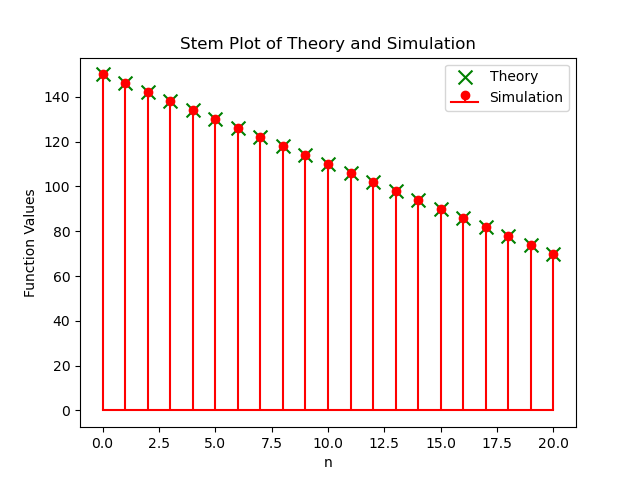
\includegraphics[width=1\linewidth]{Theory_vs_Simulation.png}
   \caption{Comparison of Theory and Simulated Values}
   \label{fig: 11.9.5.32.1}
 \end{figure}

\end{document}
